\section{Theoretische Rahmenbedinungen}

\subsection{Aktueller Forschungsstand}

\subsubsection{Definitionen}

Zunächst die Definitionen einiger Begrifflichkeiten, welche im Rahmen der Arbeit wiederholt aufgegriffen werden.\newline
\newline
\textbf{Refugees - Geflüchtete}

\begin{quote}
    \textit{Refugees are people fleeing conflict or persecution. They are defined and protected in international law, and must not be expelled or returned to situations where their life and freedom are at risk.}\cite{unhcr2017refugees}
%\caption{Definition der UNHCR}
\end{quote}
\centerline{\textit{Definition der UNHCR}}

Gemäß der Definition der Vereinten Nationen ist unter einem Geflüchteten jede Person zu verstehen, welche vor Konflikt oder Verfolgung flieht. Sie steht unter dem Schutz des internationalen Rechts und darf nicht in eine Situation entlassen werden, in der Leben oder Freiheit nicht gesichert sind.\newline

\newline
\textbf{Asylum seekers - Asylsuchende}

\begin{quote}
    \textit{An asylum-seeker is someone whose request for sanctuary has yet to be processed.}\cite{unhcr2015asylum}
%\caption{Definition der UNHCR}
\end{quote}
\centerline{\textit{Definition der UNHCR}}

Ein Asylsuchender ist eine Person, deren Antrag auf Asyl in einem Land noch nicht fertig bearbeitet wurde.

\newline
\textbf{Migrants - Migranten}

\begin{quote}
    \textit{Migrants choose to move not because of a direct threat of persecution or death, but mainly to improve their lives by finding work, or in some cases for education, family reunion, or other reasons. Unlike refugees who cannot safely return home, migrants face no such impediment to return. If they choose to return home, they will continue to receive the protection of their government.}\cite{unhcr2016migrant}
%\caption{Definition der UNHCR}
\end{quote}
\centerline{\textit{Definition der UNHCR}}

Ein Migrant zieht nicht aufgrund Verfolgung oder Lebensgefahr weiter, sondern um eine Verbesserung der Lebensbedingungen zu erreichen. Anders als Geflüchtete, deren Sicherheit am Herkunftsort nicht gewährleistet ist, genießt ein Migrant weiter den Schutz des Herkunftsstaates.
Der Akt der Migration beschreibt die Handlung, von einem Ort zu einem anderen zu ziehen - innerhalb eines Landes oder über Grenzen hinweg.

\newline
\textbf{Immigrants - Immigranten}

Ein Immigrant ist ein Migrant, welcher sich dazu entschlossen hat, permanent in einem Land zu verweilen.

\newline
\textbf{Integration}
(Halbe Definition..)
Anpassung an eine Kultur. Der Prozess, eine Person an eine Gesellschaft anzupassen. Die konkreten Mittel, um Integration von Immigranten zu erreichen, können sich je nach Kultur unterscheiden. Fast alle Konzepte von kultureller Anpassung gehen davon aus, dass die ursprünglichen Mitglieder der Gesellschaft bereits Eigenschaften miteinander teilen, die die Immigranten sich noch aneignen müssen. Anpassung an eine Kultur resultiert immer in geringerer kultureller Diversität.
\newline
\centerline{\textit{Definition der UNESCO}}


%http://www.unesco.org/new/en/social-and-human-sciences/themes/international-migration/glossary/integration/

%Providing stability to a social group: Without a certain level of integration, social organisation cannot exist. In this sense, integration includes organisational principles like the division of labour, the public celebration of solidarity, norms and rules, etc.

%Acculturation, i.e. the process of making someone equal or fitting to the rest of society. The concrete measures to produce integration of immigrants can vary according to the concept of culture that is being used. Nearly all concepts of acculturation, though, implicitly assume, that 'native' members of a host country already share the same traits which the immigrants still have to attain. Acculturation inevitably aims at reducing cultural diversity.

\textbf{Informationslücke}
\begin{center}
	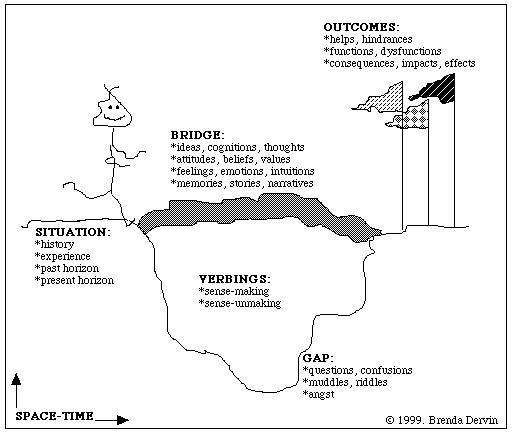
\includegraphics[scale=0.8]{SMM_MEtaphor.jpg}
	\caption{Dervin's sense-making Metapher}
\end{center}
Gemäß Brenda Dervin sind Informationslücken durch Unterschiede in Zeit \textit{(Wissenschaftlicher Fakt von heute vs Wissenschaftlicher Fakt von gestern)} und Raum \textit{(Erfahrungen einer Situation in verschiedenen Kulturen, Zusammenhängen, Gemeinschaften, materiellen Umständen, das physische Erleben einer Erfahrung und dieFormulierung dieser)} zu verstehen.\cite{dervin2003sense}

\subsubsection{Stand der Literatur}
%%%%%%%%%%%%%%%%%%%%%%%%%%%%%%%%%%%%%
%LINA'S!
%%%%%%%%%%%%%%%%%%%%%%%%%

Oduntan und Ruthven stellten 2017 im Informationsprozess von Gefl\"uchteten im Asylauswahlverfahrensprozess des Vereinigten K\"onigreichs informationsl\"ucken fest. \cite{oduntan2017investigating}
Mittels semi-strukturierter Interviews erfolgte eine Zusammenstellung verschiedener Situationen, in denen diese im Rahmen der Studie aufgedeckt wurden - mit dem Hinweis auf die Existenz noch unergr\"undeter Situationen in der Gefl\"uchtetenintegration.\newline
Informationsl\"ucken treten gem\"a\ss{} Derwin aufgrund Abweichungen in Zeit (Ich heute vs. Ich gestern) und Raum (Erfahrung aus dem Blickwinkel verschiedener Kulturen, Werte etc.) auf.\cite{dervin2003sense}\newline
Hier wurde das Informationsverhalten von sechs Gefl\"uchteten und Asylsuchenden untersucht, um Informationsbed\"urfnisse in der deutschen Fl\"uchtlingsintegration festzustellen.\newline
In der Literatur wurden bereits zahlreiche Informationsbedürfnisse und Informationslücken offengelegt:\newline
Die Informationsbedürfnisse von Migranten in Queens, NY, wurden von Fisher et al. in Sozialen, Kulturellen und Fähigkeitsbasierten Informationsbedürfnissen kategorisiert. \cite{fisher2004information}
Courtright identifizierte des weiteren medizinische Betreuung, Bildung, Wohnen und Berufstätigkeit bei Lateinamerikanischen Immigranten in Indiana, US. \cite{courtright2005health}
Silvio untersuchte südsudanesische Immigranten in Ontario, US; Ihre Informationsbedürnisse waren auf Bildung, medizinische Betreuung, Berufstätigkeit und politische Informationen bezogen, und suchten nach Mitteln und Wegen, angebracht mit Rassismus umzugehen.\cite{hakim2006information}\newline
Lloyd\cite{lloyd2014building} und Lloyd et al.\cite{lloyd2013connecting}'s Arbeit sind spezifisch auf Geflüchtete und Asylsuchende fokussiert. Lloyd ermittelte Informationsbedürfnisse im Gesundheitssektor, und Lloyd et al. entdeckte Informationsbedürfnisse im Alltag und der Anpassung an soziale Normen; beide Arbeiten beschäftigten sich mit Mündigkeit im Umgang mit Informationen.\newline
All diese Arbeiten sind Personenzentriert; es wird mit relativ kleinen Populationen gearbeitet, bei denen die Informationsbedürfnisse der Individuen untersucht werden. Ausgehend von diesen festgestellten Informationsbedürfnissen kann die Perspektive auf eine größere Population erweitert werden. So können Zusammenhänge zwischen allgemeinem menschlichem Informationsverhalten und für Geflüchtete und Asylsuchende spezifische Informationsfaktoren herstellt werden.\cite{oduntan2017investigating}\newline
Dies ist insofern wichtig, da etwa Chatman feststellte, dass sich das Informationsverhalten von Randgruppen oft signifikant von dem der Bev\"olkerungsmehrheit unterscheidet. \cite{chatman1996impoverished}
\newline
\newline 
%ICT's
Um den Integrationsprozess zu erleichtern, gab es mehrere Projekte, mit sogenannten ICT's \textit{(Information and communications technology)} die Geflüchteten zu unterstützen. Andrade et al. stellten fest, dass ICT's  f\"unf Aspekte der Gefl\"uchteten im Hinblick auf soziale Inklusion positiv beeinflussen:
\begin{enumerate}
    \item   Teilnahme an der Gesellschaft
    \item   Effizientere Kommunikation
    \item   Das Verst\"andnis der neuen Gesellschaft
    \item   Pflege sozialer Kontakte
    \item   Ausdr\"ucken einer eigenen kulturellen Identit\"at
\end{enumerate}
Diesbez\"uglich gibt es weitere Ans\"atze:\newline
Schreieck et al. etwa schufen ein Design f\"ur mobile Applikationen, das an verschiedene Kulturkreise angepasst werden kann. \cite{schreieck2017supporting}\newline
Jones et al. arbeiteten an einem anderen Ansatz: Sie kreierten ein Zuweisungssystem, in dem Gefl\"uchtete und entweder Staaten oder lokale Areale aneinander verwiesen wurden. Hierbei m\"ussen beide Parteien einer Zuweisung zustimmen. \cite{jones2017matching}\newline
Um Projekte wie diese zu verbessern, muss auch erschlossen werden, welche Informationsbed\"urfnisse die jeweiligen Zielgruppen erwarten.\newline

Durch einen Mangel an relevanten Informationen wird ein Ausschluss aus der Gesellschaft riskiert, in die die Gefl\"uchteten integriert werden sollen. \cite{andrade2016information}\newline
Als relevant werden in dieser Arbeit alle Informationen gewichtet, die das Leben in der neuen Umgebung beeinflussen - von einem Termin beim \"ortlichen Arzt \"uber Kenntnis der eigenen Rechtslage bis hin zur Grundkenntnis der \"ortlichen Kultur und Gesellschaft. \cite{schreieck2017supporting}\newline
%___________________________________________________________________________________________

In einer Studie bezüglich der Problematiken bei der
psychologischen und sozio-kulturellen Anpassung von russischsprachigen Immigranten_innen in Neuseeland zeigte sich, dass
die Motivation zur Migration einen der größten Einflüsse auf den Prozess
der Sozialisation besitzt (Maydell-Stevens, Masgoret & Ward, 2007).

Immigranten_innen stellen eine distinkte Gruppe mit spezifischen
Informationsbedürfnissen dar, mit allgemeinen Bedürfnissen zu Beginn
der Einwanderung hin zu individuellen, spezifischen Bedürfnissen im
Laufe der Integrationszeit (Shoham & Strauss, 2008).